\documentclass[tikz,border=6pt]{standalone}
\usepackage[T1]{fontenc}
\usepackage{lmodern}
\usepackage{amsmath,amssymb}
\usepackage{tikz}
\usetikzlibrary{positioning,arrows.meta,shapes.geometric,calc}

% Matched to F3.1 and style/tikz_style.tex.
\tikzset{
  bdc arrow/.style={-{Stealth[length=2.2mm,width=1.6mm]},line width=0.8pt,black},
  bdc state/.style={draw=black,line width=0.8pt,rounded corners=2pt,
    minimum width=7.5mm,minimum height=7.5mm,inner sep=1pt,font=\small},
  bdc absorbing/.style={bdc state,fill=gray!10,line width=1.0pt},
  bdc catastrophe/.style={draw=black,line width=1.0pt,ellipse,
    minimum width=9mm,minimum height=7.5mm,inner sep=1pt,font=\small,fill=gray!8},
  bdc ratelabel/.style={font=\small,inner sep=1pt,fill=white,
    fill opacity=0.88,text opacity=1},
  bdc panel title/.style={font=\bfseries\small,anchor=south},
  bdc annotation/.style={font=\small\itshape,text=black!70},
  path axis/.style={-{Stealth[length=1.8mm,width=1.3mm]},line width=0.65pt,black},
  sample path/.style={line width=1.15pt,black}
}

\newcommand{\statechain}[1]{%
  \node[bdc absorbing] (#1-zero) at (0,0) {$0$};
  \node[bdc state] (#1-one) at (1.25,0) {$1$};
  \node (#1-dots) at (2.25,0) {$\cdots$};
  \node[bdc state] (#1-n) at (3.25,0) {$n$};
  \node[bdc state] (#1-np) at (4.75,0) {$n+1$};
  \draw[bdc arrow] ([yshift=2pt]#1-n.east) --
    node[bdc ratelabel,above] {$\lambda n$} ([yshift=2pt]#1-np.west);
  \draw[bdc arrow] ([yshift=-2pt]#1-np.west) --
    node[bdc ratelabel,below] {$\mu(n+1)$} ([yshift=-2pt]#1-n.east);
  \node[bdc annotation] at (2.35,0.72)
    {$k\to k+1$ at $\lambda k$;\quad $k\to k-1$ at $\mu k$};
}

\newcommand{\sampleaxes}{%
  \draw[path axis] (0,-4.65) -- (5.4,-4.65) node[right,font=\scriptsize] {$t$};
  \draw[path axis] (0,-4.65) -- (0,-2.25) node[above,font=\scriptsize] {$X_t$};
  \node[font=\scriptsize,anchor=east] at (-0.08,-4.15) {$1$};
  \node[font=\scriptsize,anchor=east] at (-0.08,-3.60) {$2$};
  \node[font=\scriptsize,anchor=east] at (-0.08,-3.05) {$3$};
  \node[bdc annotation,anchor=south] at (2.65,-2.28) {representative sample path};
}

\begin{document}
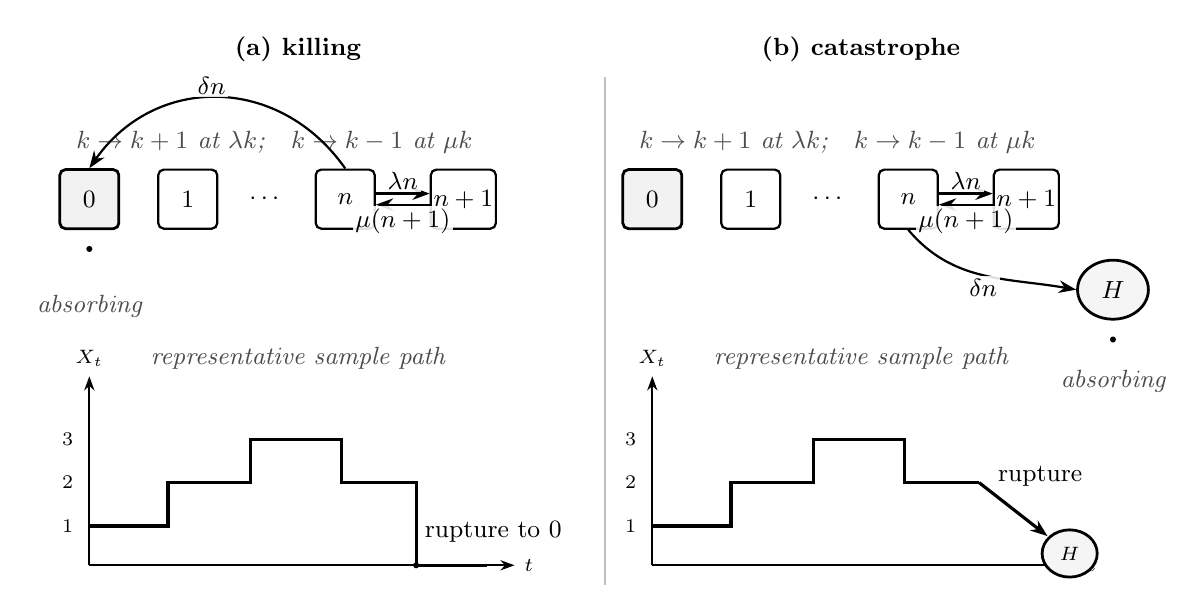
\begin{tikzpicture}[font=\small]
  % Killing convention.
  \begin{scope}[shift={(0,0)}]
    \node[bdc panel title] at (2.65,1.62) {(a) killing};
    \statechain{k}
    \draw[bdc arrow] (k-n.north) to[out=125,in=55,looseness=1.15]
      node[bdc ratelabel,above,pos=0.52] {$\delta n$} (k-zero.north);
    \node[bdc annotation,below=7mm of k-zero] {absorbing};
    \fill (k-zero.south) ++(0,-2.4mm) circle[radius=1.1pt];

    \sampleaxes
    \draw[sample path] (0,-4.15) -- (1.0,-4.15) -- (1.0,-3.60)
      -- (2.05,-3.60) -- (2.05,-3.05) -- (3.20,-3.05)
      -- (3.20,-3.60) -- (4.15,-3.60) -- (4.15,-4.65) -- (5.05,-4.65);
    \fill (4.15,-4.65) circle[radius=1.1pt];
    \node[bdc ratelabel,anchor=west] at (4.22,-4.22) {rupture to $0$};
  \end{scope}

  % Catastrophe convention.
  \begin{scope}[shift={(7.15,0)}]
    \node[bdc panel title] at (2.65,1.62) {(b) catastrophe};
    \statechain{c}
    \node[bdc catastrophe] (c-H) at (5.85,-1.15) {$H$};
    \draw[bdc arrow] (c-n.south) to[out=-50,in=170]
      node[bdc ratelabel,below,pos=0.50] {$\delta n$} (c-H.west);
    \node[bdc annotation,below=5mm of c-H] {absorbing};
    \fill (c-H.south) ++(0,-2.4mm) circle[radius=1.1pt];

    \sampleaxes
    \draw[sample path] (0,-4.15) -- (1.0,-4.15) -- (1.0,-3.60)
      -- (2.05,-3.60) -- (2.05,-3.05) -- (3.20,-3.05)
      -- (3.20,-3.60) -- (4.15,-3.60);
    \draw[bdc arrow,line width=1.15pt] (4.15,-3.60) -- (5.02,-4.28);
    \node[bdc catastrophe,minimum width=7mm,minimum height=6mm,font=\scriptsize]
      at (5.30,-4.50) {$H$};
    \node[bdc ratelabel,anchor=west] at (4.35,-3.52) {rupture};
  \end{scope}

  \draw[black!25,line width=0.6pt] (6.55,1.55) -- (6.55,-4.90);
\end{tikzpicture}
\end{document}
